\subsection{Refusal Rate Stability Analysis}
\label{sec:refusal_index_validation}


\begin{table*}[t]
    \centering
    \small
    \caption{Score stability across different refusal rates. We run evaluation with different refusal tendencies on SimpleQA for each model. $\Delta_{\text{Metric}}$ denotes the normalized difference between most-refusal and least-refusal runs. We use $p=0.2$ for the Weighted metric. Lower is better.}
    \label{tab:qwen25_simpleqa_prompt_strategies}
    \begin{tabularx}{\textwidth}{>{\raggedright\arraybackslash}p{0.12\textwidth} >{\raggedright\arraybackslash}p{0.15\textwidth} *{6}{>{\centering\arraybackslash}X}}
        \toprule
        \textbf{Type} & \textbf{Model} & \textbf{$\Delta_{\text{Accuracy}}$} & \textbf{$\Delta_{\text{Refusal}}$} & \textbf{$\Delta_{\text{C/A}}$} & \textbf{$\Delta_{\text{F-score}}$} & \textbf{$\Delta_{\text{Weighted}}$} & \textbf{$\Delta_{\text{RI}}$} \\
        \midrule
        \multirow{5}{*}{\makecell{Normalized \\ Difference}} & Mistral-123B & $-0.40$ & $+0.93$ & $+0.37$ & $-0.16$ & $-0.83$ & $\mathbf{+0.06}$ \\
         & Qwen2-35B & $-0.47$ & $+0.95$ & $+0.12$ & $-0.31$ & $-0.62$ & $\mathbf{-0.19}$ \\
         & Qwen2.5-72B & $-0.84$ & $+0.43$ & $+0.50$ & $-0.60$ & $-1.32$ & $\mathbf{-0.07}$ \\
         & Qwen3-32B & $-0.96$ & $+0.54$ & $+0.48$ & $-0.71$ & $-1.42$ & $\mathbf{+0.14}$ \\
         & Average & $-0.73$ & $+0.72$ & $+0.50$ & $-0.50$ & $-1.17$ & $\mathbf{+0.08}$ \\
        \midrule
         & \textbf{Model} & \textbf{$CV_{\text{Accuracy}}$} & \textbf{$CV_{\text{Refusal}}$} & \textbf{$CV_{\text{C/A}}$} & \textbf{$CV_{\text{F-score}}$} & \textbf{$CV_{\text{Weighted}}$} & \textbf{$CV_{\text{RI}}$} \\
        \midrule
        \multirow{5}{*}{\makecell{Coefficient of \\ Variation}} & Mistral-123B & $0.16$ & $0.35$ & $0.14$ & $0.06$ & $0.31$ & $\mathbf{0.04}$ \\
         & Qwen2-35B & $0.22$ & $0.47$ & $0.06$ & $0.14$ & $0.32$ & $\mathbf{0.09}$ \\
         & Qwen2.5-72B & $0.35$ & $0.17$ & $0.19$ & $0.26$ & $0.53$ & $\mathbf{0.03}$ \\
         & Qwen3-32B & $0.35$ & $0.19$ & $0.17$ & $0.28$ & $0.51$ & $\mathbf{0.07}$ \\
         & Average & $0.29$ & $0.29$ & $0.19$ & $0.21$ & $0.46$ & $\mathbf{0.08}$ \\
        \bottomrule
    \end{tabularx}
\end{table*}


In this section, we validate the Refusal Index and analyze its stability across different refusal rates. 
We demonstrate that: (1) the Refusal Index conceptualizes and evaluates the model's knowledge-aware refusal with an \emph{accuracy-refusal curve}, and (2) the two-pass evaluation returns consistent RI across different refusal rates.

\paragraph{RI Measures Knowledge-aware Refusal with Accuracy-Refusal Curve}
An accuracy-refusal curve measures knowledge-aware refusal by showing the correct answer rate at each refusal rate for a model on the same dataset.
While refusing more uncertain questions reduces incorrect answers, it also leads to fewer correct answers due to false refusals. 
By varying the overall refusal rate, each model exhibits a trade-off between correct answers and refusal rate. 
As shown in Figure~\ref{fig:acc_rej_plot_with_contour_lines}, fixing any metric constant gives a unique iso-score curve in the accuracy–refusal plane, which describes the accuracy-refusal trade-off relationship assumed by the metric.

\begin{wrapfigure}{r}{0.48\textwidth}
    \centering
    \vspace{-1.5em}
    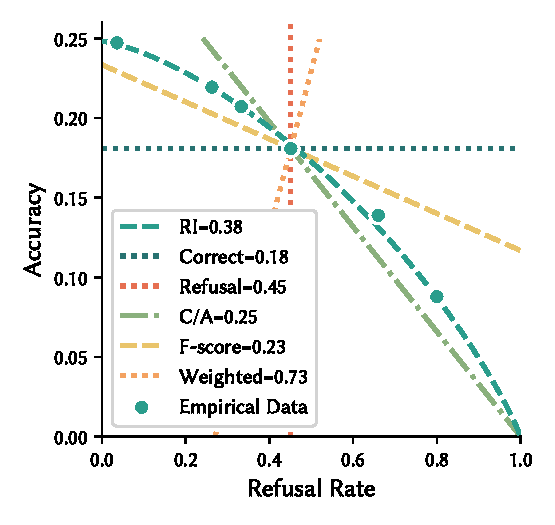
\includegraphics[width=0.48\textwidth]{Figures/acc_rej_plot_with_contour_lines.pdf}
    \caption{Comparison of factuality metrics with iso-score accuracy-refusal trade-off curves. C/A, F, and W correspond to Correct / Attempted, F-score, and Weighted score, respectively.}
    \vspace{-1em}
    \label{fig:acc_rej_plot_with_contour_lines}
\end{wrapfigure}


Compared with heuristic metrics, iso-RI curves have two desirable properties: (1) they represent sensible accuracy–refusal trade-offs matching the expected behavior of the model (see Figure~\ref{fig:refusal_index_illustration}, left). 
Different iso-RI curves yield the same maximum correct answer number when the refusal rate is 0 and reach zero correct answers when the refusal rate is 1; and (2) RI is agnostic to the maximum correct answer number and refusal rate, controlling only the convexity of the curve and capturing how well a model preserves correct answers by reducing false refusals. 
That is, for two models with the same maximum correct answer number, the one with higher RI retains more correct answers when refusing the same fraction of questions. 
In contrast, heuristic metrics fail to capture this property, imposing approximately linear accuracy–refusal relationships at fixed scores. 
In summary, the Refusal Index does not simply reward higher correct answer rate or lower refusal rates, but captures the level of rank calibration in refusal decisions, distinct from all previous metrics.

% \begin{figure}[t]
%     \centering
%     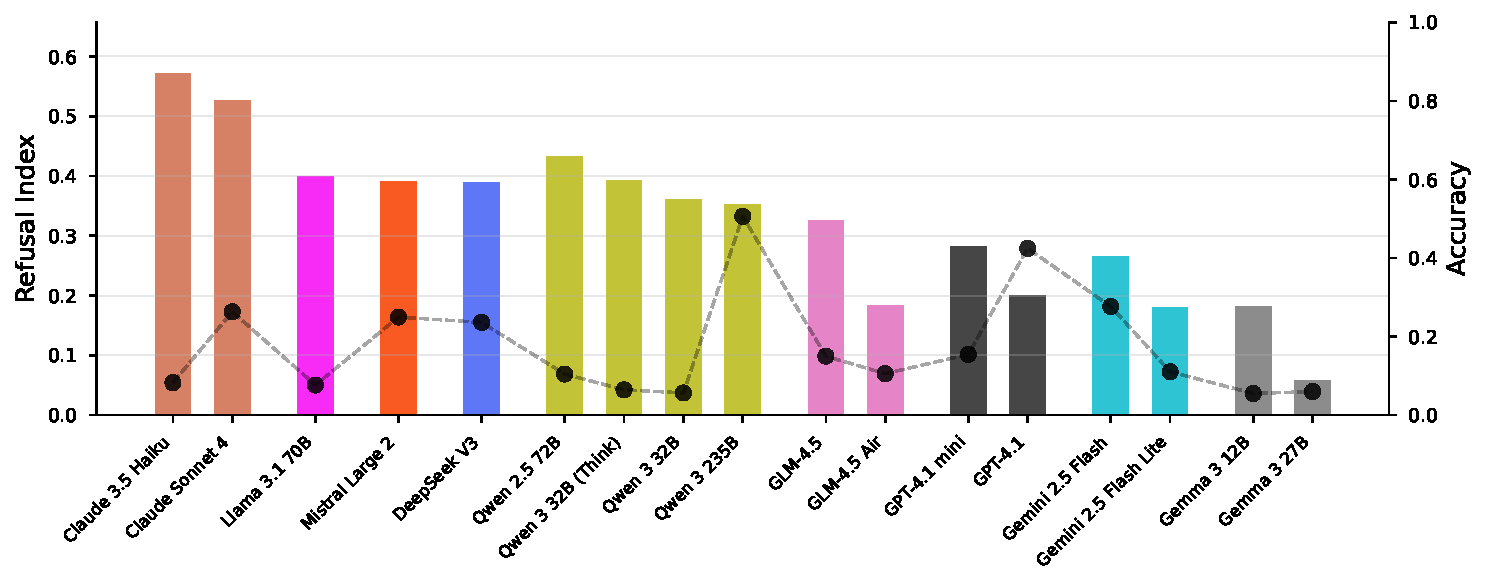
\includegraphics[width=0.95\linewidth]{Figures/simpleqa_refusal_index.pdf}
%     \caption{Evaluation results of the Refusal Index on SimpleQA. }
%     \label{fig:simpleqa_refusal_index}
% \end{figure}

\paragraph{RI remains consistent across different refusal rates.}
To empirically validate RI, we test whether the Refusal Index remains consistent across different refusal rates. 
For this, we design a set of system prompts that progressively encourage caution in answering to induce different refusal rates, then apply them to the same model on the SimpleQA dataset. 
Our results demonstrate that RI exhibits remarkable stability across these different refusal rates, while heuristic metrics show substantial variation. 
As shown in Table~\ref{tab:qwen25_simpleqa_prompt_strategies}, RI exhibits approximately 70\% lower variability compared to heuristic metrics. 
This empirical finding suggests that prompt-induced changes in refusal rate shift the refusal probability distribution without changing the correlation between refusal probability and error probability. 
In the appendix, we provide additional validation through goodness-of-fit tests for the Gaussian copula assumption.


\subsection{Alignment with Calibration Methods}

\paragraph{RI is highly consistent with sampling-based calibration methods.}
One potential concern with RI is that although it is defined as the rank correlation between refusal probability and error probability, the two-pass evaluation may not faithfully reflect that correlation. 
To address this, we compare RI values with AUROC scores computed using P(Answering) as an uncertainty estimation method. 
We choose AUROC with P(Answering) for a fair comparison because it shares the same definition of uncertainty as RI. 
Specifically, (1) AUROC is a rank-calibration metric that only measures the discriminative ability of refusal and (2) P(Answering) is a direct estimation of the prediction probability for model refusals. 
While there exist other calibration metrics like ECE, Brier Score, and various uncertainty estimation methods, AUROC with P(Answering) is the most direct measurement of the correlation between refusal and error.
\Figref{fig:comparison_auroc} shows the results. 
Among the evaluated metrics, RI demonstrates the strongest positive correlation with AUROC at 85\%, outperforming all other metrics.
This high agreement between RI and AUROC with P(Answering) suggests that RI accurately reflects the correlation between refusal probability and error probability.
Meanwhile, RI requires much smaller computational overhead compared to estimating P(Answering) with multiple sampling.


\begin{figure}[t]
    \centering
    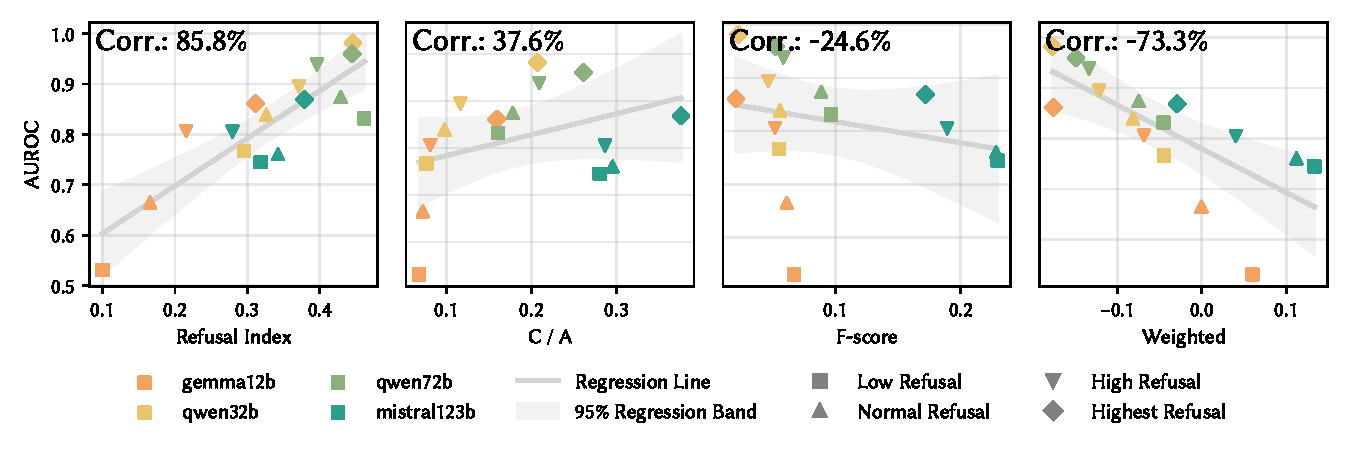
\includegraphics[width=\linewidth]{Figures/comparison_auroc_panswer.pdf}
    \caption{Correlation between factuality metrics and AUROC with P(Answering) on SimpleQA. RI shows the highest positive correlation with AUROC while being orders of magnitude cheaper to compute.}
    \label{fig:comparison_auroc}
\end{figure}

\subsection{Model Ranking Stability}

Finally, we study whether the knowledge-aware refusal measured by RI is consistent across different models and datasets. 
To this end, we measure model ranking stability: does RI rank models consistently in different datasets or evaluation settings? 
Higher ranking stability suggests that a metric captures genuine, discriminative properties of models. 
Specifically, we calculate Kendall's $W$ (overall ranking agreement) and Winner Entropy (top-1 consistency) on all 8 evaluation settings (4 refusal-varying evaluations on SimpleQA + 4 hallucination benchmarks). 
Additionally, to capture the ranking stability of the correlation structure between correct answers and refusals, we want to filter out the sole effect from the correct answer rate or refusal rate. 
We make the removal by performing an isotonic regression on the correct answer rate or refusal rate across different setups for each model, then remove the regressed values from each metric. We calculate the Kendall's $W$ and Winner Entropy on the residuals, effectively measuring parts of the metric that cannot be explained by correct answer rate or refusal rate alone.

\paragraph{RI provides stable model rankings independent of accuracy and refusal rate.} 
As shown in Table~\ref{tab:ranking_stability}, when removing the monotonic effect of correct answer rate or refusal rate, RI still shows high ranking stability, while heuristic metrics degrade to near random values. 
We can see that heuristic metrics like F-score and Weighted achieve very good ranking stability, but their Kendall's $W$ and Winner Entropy drop quickly when we remove the monotonic effect from correct answer rate or refusal rate. 
This result suggests that while heuristic metrics like F-score have high ranking stability, they are mostly explained by correct answer rate or refusal rate. 
In contrast, RI retains most of its ranking stability even after removing the effects from correct answer rate and refusal rate, indicating that it captures the intrinsic knowledge-aware refusal of models, persisting across different evaluation settings.


\begin{table}[t]
    \centering
    \small
    \caption{Ranking stability across different evaluation settings. $-\text{Correct}$ and $-\text{Refusal}$ show results after removing monotonic effects of correct answer rate and refusal rate with isotonic regression. $- \text{Both}$ removes both correctness and refusal rates with additive isotonic regression.}
    \label{tab:ranking_stability}
    \setlength{\tabcolsep}{4pt}
    \begin{tabular}{lcccccccc}
        \toprule
         & \multicolumn{4}{c}{\textbf{Kendall's W} $\uparrow$} & \multicolumn{4}{c}{\textbf{Winner Entropy} $\downarrow$} \\
        \cmidrule(lr){2-5} \cmidrule(lr){6-9}
        \textbf{Metric} & \textbf{Default} & \textbf{$- \text{Correct}$} & \textbf{$- \text{Refusal}$} & \textbf{$- \text{Both}$} & \textbf{Default} & \textbf{$- \text{Correct}$} & \textbf{$- \text{Refusal}$} & \textbf{$- \text{Both}$} \\
        \midrule
        Random Value  & 0.25 & 0.25 & 0.25 & 0.25 & 0.61 & 0.61 & 0.61 & 0.61 \\
        Correct Answer Rate & 0.87 & 0.00 & \textbf{0.48} & 0.39 & \textbf{0.00} & 1.00 & 0.48 & 1.00 \\
        Refusal Rate & 0.86 & 0.44 & 0.00 & 0.30 & 0.18 & 0.61 & 1.00 & 1.00 \\
        \midrule
        C / A    & 0.69 & \textbf{0.63} & 0.40 & 0.37 & 0.33 & 0.61 & 0.48 & 0.61 \\
        F-score  & \textbf{0.90} & 0.10 & 0.48 & 0.39 & 0.00 & \textbf{0.18} & 0.48 & 0.52 \\
        Weighted & 0.87 & 0.60 & 0.25 & 0.32 & 0.33 & 0.33 & \textbf{0.37} & 0.61 \\
        RI       & 0.47 & 0.50 & 0.35 & \textbf{0.49} & 0.47 & 0.33 & 0.61 & \textbf{0.37} \\
        \bottomrule
    \end{tabular}%
    \\
\end{table}